%%
%% Copyright 2007, 2008, 2009 Elsevier Ltd
%%
%% This file is part of the 'Elsarticle Bundle'.
%% ---------------------------------------------

\documentclass[preprint,12pt, a4paper]{elsarticle}

%% The amssymb package provides various useful mathematical symbols
\usepackage{amssymb}
\usepackage{hyperref}
\usepackage{listings}
\usepackage{xcolor}
\usepackage{graphicx}

\setlength{\parindent}{0pt}

% Code listing style
\lstset{
  language=Python,
  basicstyle=\ttfamily\small,
  keywordstyle=\color{blue},
  stringstyle=\color{red},
  commentstyle=\color{green!60!black},
  frame=single,
  breaklines=true,
  showstringspaces=false
}

\journal{SoftwareX}

\begin{document}
\renewcommand{\labelenumii}{\arabic{enumi}.\arabic{enumii}}

\begin{frontmatter}

\title{EnerHabitat: A Python package and web application for the time-dependent thermal evaluation of homogeneous and non-homogeneous building envelope components}

\author[ier]{M. Cruz Salas}
\author[ipn]{F. Rodr\'iguez Calder\'on}
\author[ier]{G. Huelsz}
\author[ier]{J. Rojas}
\author[ier]{G. Barrios\corref{cor1}}
\ead{gbv@ier.unam.mx}

\cortext[cor1]{Corresponding author}

\address[ier]{Instituto de Energ\'ias Renovables, Universidad Nacional Aut\'onoma de M\'exico, Priv. Xochicalco s/n, Col. Centro, 62580 Temixco, Mor., Mexico}
%% TODO: afiliacion completa de Fernando (unidad del IPN y direccion postal) -- pendiente
\address[ipn]{Instituto Polit\'ecnico Nacional, Mexico}

\begin{abstract}
EnerHabitat is an open-source Python package and web application for evaluating the time-dependent thermal performance of building envelope walls and roofs. It solves time-dependent heat transfer through multilayer constructive systems, in one dimension for homogeneous layers and in two dimensions for non-homogeneous units such as joist-and-block roofs with air cavities. It uses an implicit finite control volumes accelerated with Numba, with solar boundary conditions computed from standard EPW weather files via pvlib. Both free-running and air-conditioned indoor conditions are supported. EnerHabitat succeeds a validated Java-based web tool that performed over one million evaluations; the web application makes the model accessible to users without programming experience.
\end{abstract}

\begin{keyword}
building envelope \sep thermal performance \sep time-dependent heat transfer \sep non-homogeneous constructive systems \sep Python \sep EPW
\end{keyword}

\end{frontmatter}

%% Metadata Tables
\section*{Required Metadata}
\label{sec:metadata}

\section*{Current code version}

\begin{table}[!h]
\begin{tabular}{|l|p{6.5cm}|p{6.5cm}|}
\hline
\textbf{Nr.} & \textbf{Code metadata description} & \textbf{Metadata} \\
\hline
C1 & Current code version & v0.2.1 \\
\hline
C2 & Permanent GitHub link to code/repository used for this code version & \url{https://github.com/Ener-Habitat/EnerHabitat/tree/v0.2.1} \\
\hline
C3 & Legal Code License & MIT License \\
\hline
C4 & Code versioning system used & git \\
\hline
C5 & Software code languages, tools, and services used & Python, numba, pvlib, pandas, numpy \\
\hline
C6 & Compilation requirements, operating environments \& dependencies & Python $\geq$ 3.10, numba $\geq$ 0.62.1, pvlib $\geq$ 0.13.1; Windows, Linux, macOS \\
\hline
C7 & If available Link to developer documentation/manual & \url{https://ener-habitat.github.io/EnerHabitat/} \\
\hline
C8 & Support email for questions & gbv@ier.unam.mx \\
\hline
\end{tabular}
\caption{Code metadata (mandatory)}
\label{codeMetadata}
\end{table}

\section{Motivation and significance}

The thermal behavior of opaque building envelopes---walls and roofs---plays a central role in the energy consumption and indoor comfort of buildings, particularly in warm climates and in free-running (non-air-conditioned) dwellings where mechanical cooling is absent or unaffordable. Nevertheless, in many regulatory frameworks and design tools, envelope components are still characterized by steady-state indicators such as U-values or R-values \cite{ashrae2021fundamentals}. These indicators neglect thermal mass and the dynamic interaction between solar gains, outdoor temperature cycles, and heat storage, and can therefore mislead design decisions, especially for lightweight or non-homogeneous constructions in regions with strong diurnal temperature swings and high solar irradiation \cite{barrios2011wall,barrios2012envelope}. Key time-dependent performance parameters include the decrement factor (the ratio of indoor to outdoor temperature amplitude), the time lag (the delay between outdoor and indoor temperature peaks), and the energy transferred through the component \cite{barrios2012envelope}.

Several families of tools relate to this problem. Whole-building simulation programs such as EnergyPlus \cite{energyplus} and TRNSYS provide detailed dynamic modelling of entire buildings, but require significant expertise and complex input structures \cite{crawley2008contrasting}, and they are not optimized for the rapid exploration of single envelope components. Steady-state calculators focus on U-values and thus cannot capture the attenuation and time lag of heat waves through walls and roofs. Two- and three-dimensional conduction tools such as THERM or HEAT2 represent thermal bridges and non-homogeneous details, but they are typically used in steady-state or harmonic regimes and do not provide the envelope-oriented dynamic metrics needed by designers in warm climates.

The original Ener-Habitat addressed this gap as a Java-based web application implementing time-dependent models for single envelope components, capable of handling homogeneous multilayer systems as well as systems including a non-homogeneous layer with air cavities, under air-conditioned or free-running indoor conditions, for several Mexican cities \cite{barrios2016enerhabitat}. The models were validated against EnergyPlus for homogeneous assemblies, with maximum temperature differences of 0.5$^\circ$C, and against hot-box experiments for hollow concrete block walls \cite{barrios2016enerhabitat}; the tool was also used to propose thermal performance parameters tailored to free-running buildings \cite{barrios2011wall,barrios2012envelope}. Internal usage records registered over one million thermal evaluations during its roughly ten years of operation (these logs are no longer archived). The tool was eventually discontinued due to the burden of maintaining its Java web infrastructure: it was closed-source, restricted to a predefined climate database, and offered no possibility of automation, extension, or integration into scientific workflows.

The new EnerHabitat re-implements these validated models as an open-source ecosystem: (1) a Python package distributed via PyPI that exposes the one-dimensional and two-dimensional solvers for programmatic use in parametric studies and computational workflows; (2) a web application built with Shiny for Python that provides a graphical interface to the one-dimensional model for users without programming experience; and (3) a public validation repository with executable notebooks. All components are released under the MIT license, and the use of standard EnergyPlus Weather (EPW) files extends the applicability worldwide, beyond the original Mexican focus. This design directly addresses several needs: it provides an accessible reference implementation of time-dependent heat transfer in multilayer envelopes with convective boundary conditions; it allows researchers and designers to systematically explore how material choices, layer ordering, and non-homogeneous geometries affect dynamic metrics; and it supports the development of evaluation criteria beyond steady-state indicators for building energy standards such as Mexico's NOM-020-ENER \cite{nom020ener}.

From the user's perspective, a typical workflow consists of: (i) selecting an EPW file and an analysis month; (ii) defining one or more constructive systems as ordered layer sequences, optionally including one non-homogeneous element; (iii) choosing the component position (wall or roof), tilt, and orientation; (iv) selecting free-running or air-conditioned indoor conditions; and (v) running the simulation to obtain the temperature time series and summary performance indicators.


\section{Software description}

\subsection{Software architecture}

EnerHabitat is distributed as an open-source ecosystem of three coupled components (Figure~\ref{fig:architecture}): the \texttt{enerhabitat} Python package \cite{enerhabitat_v021}, which is the computational core, available on PyPI; a web application that provides a graphical interface to the one-dimensional model---including derived metrics such as the decrement factor, cooling and heating energy analysis under air conditioning, and time-series export (source code at \url{https://github.com/Ener-Habitat/EnerHabitat-webapp}); and a validation repository with executable notebooks, described in Section~\ref{sec:examples}.

The Python package is organized around four main classes:

\begin{itemize}
    \item \textbf{Location}: Handles EnergyPlus Weather (EPW) file parsing and climate data processing. It extracts metadata (city, latitude, longitude, altitude, timezone) and computes the mean day of any specified month, using pvlib \cite{anderson2023pvlib} for solar position and irradiance calculations.

    \item \textbf{System}: Represents a homogeneous multilayer constructive system (wall or roof). It manages the layer definitions---an ordered list of (material, thickness) pairs, listed from the outdoor to the indoor surface, as in EnergyPlus---, the surface properties (tilt, azimuth, solar absorptance), the sol-air temperature calculation, and the one-dimensional heat transfer solvers.

    \item \textbf{System2D}: Mirrors the \texttt{System} interface for constructive systems that include one non-homogeneous element: a \texttt{HollowBlock} (hollow concrete block, for walls) or a \texttt{Slab} (joist-and-block roof), whose cross-sections contain air cavities. The cavity physics couples surface-to-surface radiation, computed with view factors, and temperature-dependent Nusselt convection with a lumped cavity-air node. Cavities can alternatively be filled with a solid material.

    \item \textbf{Config}: Provides global configuration management, including the material properties database (an editable INI file), the discretization parameters, and the convective heat transfer coefficients.
\end{itemize}

The solvers discretize the transient heat conduction equation with an implicit finite control volume scheme \cite{patankar1980numerical} solved with the Tridiagonal Matrix Algorithm (TDMA), and the mean day is iterated until the solution becomes periodic. Performance-critical loops are compiled just-in-time with Numba \cite{lam2015numba}, so one-dimensional simulations complete within seconds on a laptop, while two-dimensional solutions with the default mesh take on the order of tens of minutes.

The web application is built with Shiny for Python \cite{shiny2024python} as a thin, stateless presentation layer: the interface callbacks collect user input, call the \texttt{enerhabitat} package, and render the results as interactive Plotly \cite{plotly2024python} visualizations. All computation is delegated to the package, which keeps the application easy to maintain.

\begin{figure}[t]
\centering
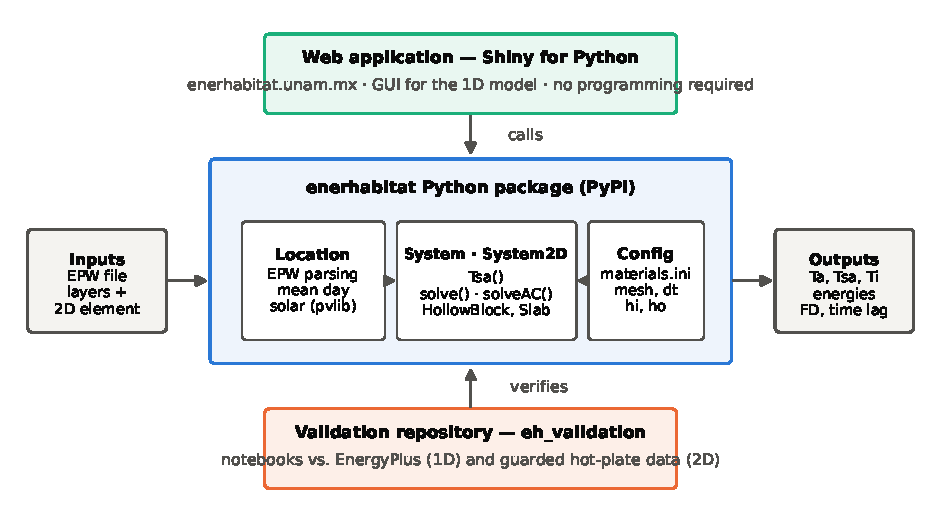
\includegraphics[width=0.95\textwidth]{figures/Figure_1.pdf}
\caption{The EnerHabitat ecosystem. The \texttt{enerhabitat} Python package is the computational core, organized around the \texttt{Location}, \texttt{System}/\texttt{System2D}, and \texttt{Config} classes; the Shiny for Python web application provides a graphical interface to the one-dimensional model; and the validation repository verifies the solvers against EnergyPlus and against published guarded hot-plate measurements.}
\label{fig:architecture}
\end{figure}

\subsection{Software functionalities}

\subsubsection{Python package functionalities}

\textbf{Climate data processing}: The \texttt{Location} class reads EPW files and computes the mean day of the selected month, including the ambient temperature, the global, beam, and diffuse irradiance components, and the neutrality temperature of the adaptive comfort model \cite{humphreys2000outdoor}.

\textbf{Sol-air temperature}: The \texttt{Tsa()} method computes the sol-air temperature experienced by the surface, accounting for its tilt and azimuth, its solar absorptance, the outdoor convection coefficient, and the long-wave radiation correction for horizontal surfaces (roofs).

\textbf{Heat transfer solution}: Two solution modes are available, with the same interface in the one- and two-dimensional solvers:
\begin{itemize}
    \item \texttt{solve()}: Solves the free-running case, in which no air conditioning is present. The indoor air, modeled as a lumped thermal mass, responds freely to the heat transferred through the envelope component, and the energy delivered to it over the mean day is reported.
    \item \texttt{solveAC()}: Holds the indoor air at the neutrality temperature (air-conditioned case) and reports the cooling and heating energies required to maintain it.
\end{itemize}

\textbf{Non-homogeneous systems}: A \texttt{System2D} accepts one \texttt{HollowBlock} or \texttt{Slab} element at any position of the layer stack. The cross-section geometry of the element (rib, filler block, compression topping, number and size of cavities) is fully parametric, and each cavity can contain air or a solid fill material. A section inspector renders the discretized cross-section to scale for visual verification before solving.

\textbf{Output metrics}: The solvers return the time series of the outdoor, sol-air, and indoor temperatures over the mean day; the reported energies are expressed per unit of interior area and per mean day (J/m$^2$). Additional metrics, such as the decrement factor and the time lag, can be derived from the temperature time series.

\subsubsection{Web application functionalities}

The web application exposes the one-dimensional model through an accessible interface with the following features:

\textbf{Multiple system comparison}: Users can evaluate up to 5 constructive systems simultaneously, enabling direct comparison of different design alternatives.

\textbf{Flexible configuration}: The interface supports 8 surface orientations (N, NE, E, SE, S, SW, W, NW) and wall (90$^\circ$) or roof (0$^\circ$) inclinations. Each system can have up to 10 layers with independent material and thickness specifications.

\textbf{Interactive visualization}: Temperature plots show ambient temperature, sol-air temperature, and indoor temperature for each system, with a shaded comfort zone band. Energy mode displays stacked bar charts comparing cooling and heating requirements across systems.

\textbf{Metrics display}: A summary table presents key performance metrics including decrement factor (FD), time lag (TR), and energy transfer (ET) for each evaluated system.

\textbf{Data export}: Results can be downloaded as CSV files for further analysis in external tools.


\section{Illustrative examples}
\label{sec:examples}

\subsection{Example 1: Python package usage}

The following code demonstrates basic usage of the EnerHabitat package to evaluate a two-layer wall system:

\begin{lstlisting}[caption={Evaluation of a two-layer wall with the EnerHabitat Python package (1D)}]
import enerhabitat as eh

# Materials database (thermal conductivity, density, specific heat)
eh.config.file = "materials.ini"

# Location from an EPW weather file; mean day of May
loc = eh.Location("Cuernavaca.epw")
loc.info()   # city, timezone, latitude, longitude, altitude
mean_day = loc.meanDay(month="5")

# South-facing wall, layers from outside to inside:
# 1 in (0.0254 m) EPS insulation + 12 cm concrete
wall = eh.System(location=loc, tilt=90, azimuth=180)
wall.absortance = 0.7
wall.layers = [("EPS", 0.0254), ("Concrete", 0.12)]

# Sol-air temperature at the outdoor surface
tsa = wall.Tsa()

# Free-running indoor temperature (no air conditioning)
ti = wall.solve()
print(f"Energy transfer: {wall.energy_transfer:.0f} J/m2 per day")

# Air-conditioned mode: energy to hold the neutrality temperature
wall.solveAC()
print(f"Cooling energy: {wall.cooling_energy:.0f} J/m2 per day")
print(f"Heating energy: {wall.heating_energy:.0f} J/m2 per day")
\end{lstlisting}

Figure~\ref{fig:meanday1d} shows the result: placing one inch of insulation on the outdoor side of the concrete wall reduces the free-running indoor temperature swing from about 14$^\circ$C to 2$^\circ$C---behavior that time-dependent analysis reveals and steady-state indicators cannot capture.

\begin{figure}[t]
\centering
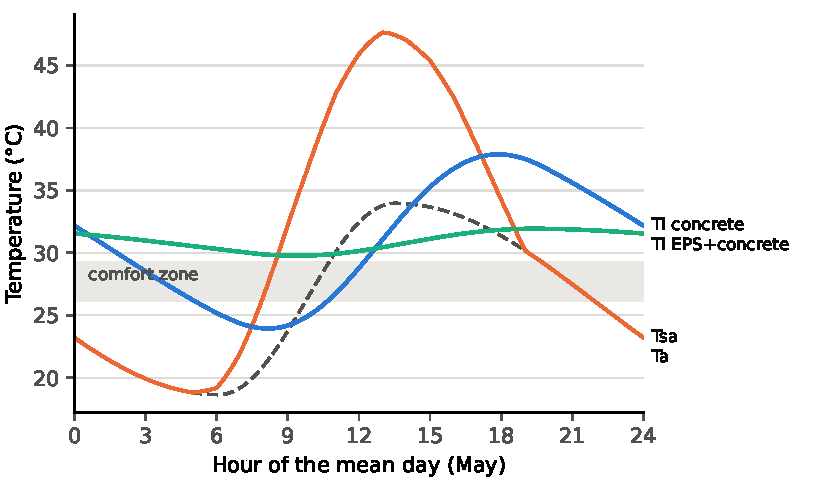
\includegraphics[width=0.9\textwidth]{figures/Figure_2.pdf}
\caption{Mean-day temperatures computed by Listing~1 for a south-facing wall in Cuernavaca, Mexico, in May (solar absorptance 0.7): outdoor air temperature ($T_a$), sol--air temperature ($T_{sa}$), and free-running indoor air temperature ($T_i$) for the 12 cm concrete wall with and without 1 in of exterior EPS insulation. The shaded band is the adaptive comfort zone.}
\label{fig:meanday1d}
\end{figure}

\subsection{Example 2: A joist-and-block roof with air cavities (2D)}

Listing~2 evaluates a joist-and-block roof (\textit{vigueta y bovedilla}), a constructive system widely used in Mexican housing: an L-shaped high-density concrete joist, lightweight filler blocks surrounding three air cavities, and an aerated-concrete compression topping, waterproofed on the outside and plastered on the inside. The cross-section geometry is fully parametric; Figure~\ref{fig:slab} shows the section as drawn by the package's inspector.
With the default mesh, this simulation converges after eleven iterated mean days in about 21 minutes on a laptop; the energy delivered to the indoor air is 11{,}539 J/m$^2$ per day.

Figure~\ref{fig:slabresult} shows the resulting mean day: the indoor temperature swing is damped to about 4$^\circ$C, and at night the sol--air temperature drops below the ambient temperature because of the long-wave radiative exchange between the horizontal surface and the sky.

\begin{figure}[t]
\centering
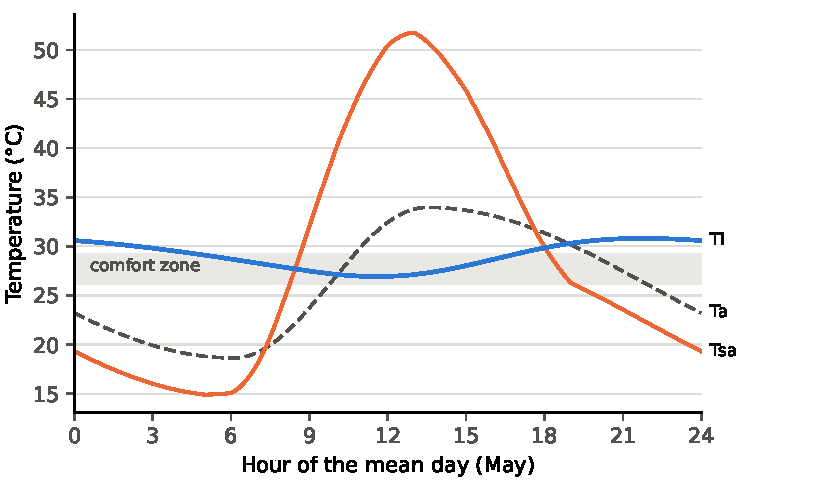
\includegraphics[width=0.9\textwidth]{figures/Figure_4.pdf}
\caption{Mean-day result of Listing~2 for the joist-and-block roof in Cuernavaca, Mexico, in May (solar absorptance 0.3): outdoor air temperature ($T_a$), sol--air temperature ($T_{sa}$), and free-running indoor air temperature ($T_i$). At night $T_{sa}$ falls below $T_a$ owing to the long-wave radiation exchange with the sky; the shaded band is the adaptive comfort zone.}
\label{fig:slabresult}
\end{figure}

\begin{figure}[t]
\centering
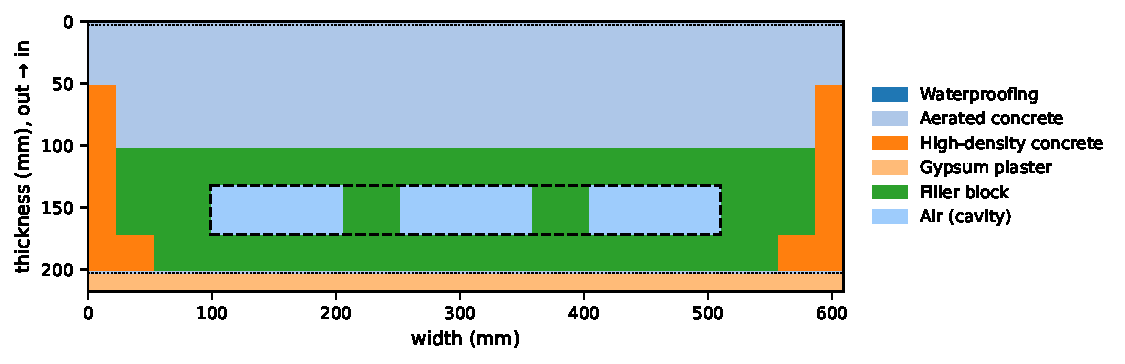
\includegraphics[width=0.95\textwidth]{figures/Figure_3.pdf}
\caption{The joist-and-block roof of Listing~2, drawn to scale by the package's section inspector (\texttt{preview()}): an L-shaped high-density concrete joist, lightweight filler blocks (\textit{bovedilla}) surrounding three air cavities, an aerated-concrete compression topping, waterproofing on the outside, and gypsum plaster on the inside. The legend labels are the material entries used in Listing~2.}
\label{fig:slab}
\end{figure}

\begin{lstlisting}[caption={Evaluation of a joist-and-block roof with the 2D solver}]
import enerhabitat as eh

eh.config.file = "materials.ini"

slab = eh.Slab(
    rib_material     = "High-density concrete",  # L-shaped joist (web + foot)
    block_material   = "Filler block",           # bovedilla, surrounds cavities
    topping_material = "Aerated concrete",       # compression topping
    fill_type        = eh.Fill.AIR,              # air cavities (or eh.Fill.SOLID)
    emissivity       = 0.9,
    geometry = {
        "web": 0.025, "foot": 0.025, "shoulder": 0.050,
        "n_cavities": 3, "cavity_width": 0.103,
        "topping": 0.100, "topping_cap": 0.050,
        "cover_top": 0.030, "cavity": 0.040, "cover_bottom": 0.030,
    },
)

roof = eh.System2D(eh.Location("Cuernavaca.epw"))
roof.tilt = 0                 # horizontal surface: roof
roof.absortance = 0.3
roof.layers = [("Waterproofing", 0.003), slab, ("Gypsum plaster", 0.015)]  # outside -> inside
roof.location.meanDay(month="5")
roof.Tsa()

roof.solve()                  # free-running; or roof.solveAC()
print(f"Energy transfer: {roof.energy_transfer:.0f} J/m2 per day")
\end{lstlisting}

\subsection{Example 3: Validation}

The validation repository (\url{https://github.com/Ener-Habitat/eh_validation}) contains the EPW files, the EnergyPlus models, the experimental reference data, and Jupyter notebooks that reproduce each validation case:

\begin{itemize}
    \item \textbf{1D versus EnergyPlus}: free-running and air-conditioned mean-day simulations of five 10-cm homogeneous walls (adobe, fired-clay brick, concrete, expanded polystyrene, and a compressed adobe composite) in Temixco, Mexico. The results are consistent with the original validation \cite{barrios2016enerhabitat}, which reported maximum temperature differences of 0.5$^\circ$C, decrement factor differences of 0.03, time lag differences of 0.4 h, and energy differences within 4\%.
    \item \textbf{2D internal consistency}: a hollow block whose cavities are filled with the same material as its shell becomes a solid block, and its indoor temperature series reproduces that of the equivalent homogeneous 1D wall.
    \item \textbf{2D versus experiment}: the hollow concrete block with air cavities is validated against the thermal resistance measured experimentally by Borb\'on et al. \cite{borbon2010} with a guarded hot plate (ASTM C177), reproducing the reported dependence of the resistance on the temperature difference across the wall and on its mean temperature, and including a mesh convergence study and a sensitivity analysis of the cavity emissivity.
\end{itemize}

\subsection{Example 4: Web application workflow}

The web application at \url{https://enerhabitat.unam.mx} enables users to:

\begin{enumerate}
    \item Select or upload an EPW weather file and choose the analysis month
    \item Configure surface geometry (wall/roof, orientation)
    \item Define up to 5 constructive systems by adding layers with materials and thicknesses
    \item Toggle between temperature analysis (without A/C) and energy analysis (with A/C) modes
    \item View interactive plots comparing system performance
    \item Export results as CSV for further analysis
\end{enumerate}

The interface displays temperature time series with comfort zone bands for non-air-conditioned analysis, or stacked bar charts showing cooling and heating requirements for air-conditioned analysis. Figure~\ref{fig:webapp} shows an air-conditioned evaluation of three constructive systems for an east-facing wall in Cuernavaca, Mexico, in May. The interface is in Spanish, the native language of the authors and of the tool's primary user community.

\begin{figure}[t]
\centering
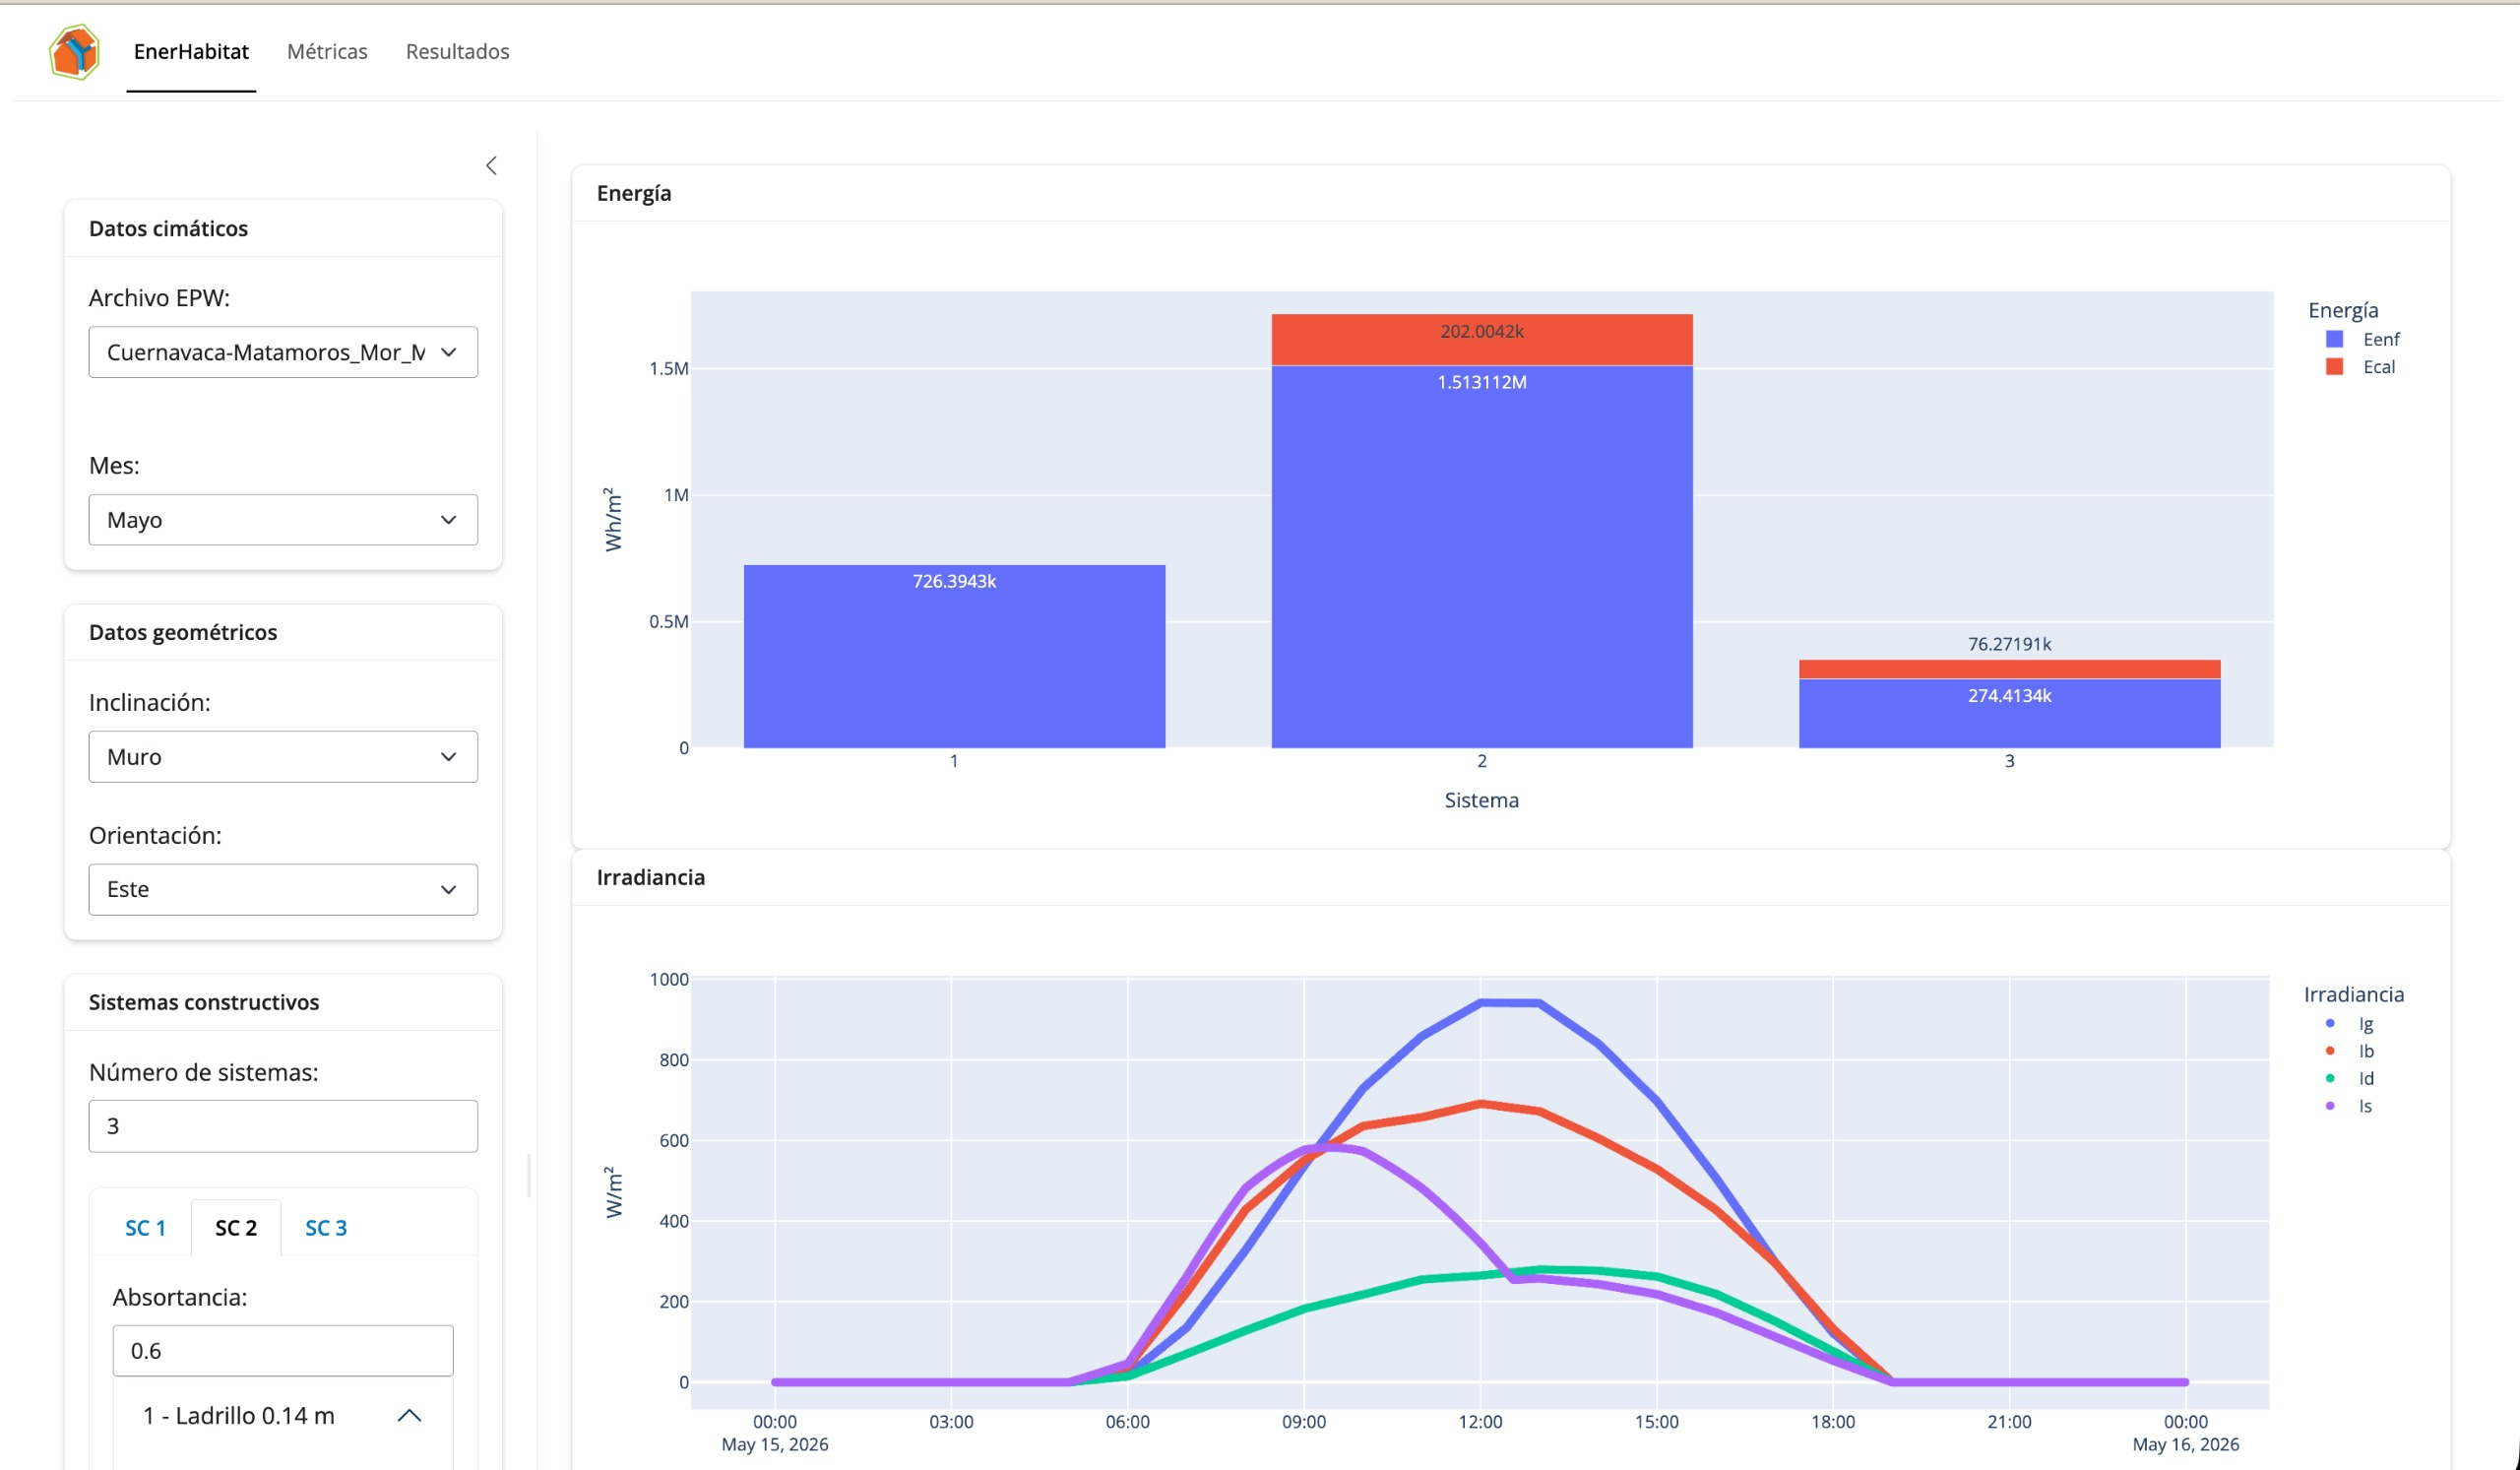
\includegraphics[width=0.95\textwidth]{figures/Figure_5.png}
\caption{The EnerHabitat web application (\url{https://enerhabitat.unam.mx}) evaluating three constructive systems for an east-facing wall in Cuernavaca, Mexico, in May, in air-conditioned mode. The stacked bars show the cooling (\textit{Eenf}) and heating (\textit{Ecal}) energies of each system, and the lower panel shows the global, beam, diffuse, and surface irradiances of the mean day. The interface is in Spanish, the native language of the authors and of the tool's primary user community.}
\label{fig:webapp}
\end{figure}


\section{Impact}

EnerHabitat targets the long-standing gap between detailed whole-building simulators and simple steady-state calculators: a lightweight, envelope-centric tool that captures the time-dependent behavior of walls and roofs under realistic solar and temperature forcing, including non-homogeneous units with air cavities, for both air-conditioned and free-running buildings \cite{barrios2016enerhabitat}.

\textbf{New research questions}: Because the numerical core is an ordinary Python package, questions that were impractical through the original web form can now be explored programmatically: systematic sweeps of material substitutions, layer ordering, and cavity geometries, and their effect on dynamic metrics such as the decrement factor, the time lag, and the heating and cooling loads; the development and testing of envelope performance indicators beyond the steady-state U-value, tailored to warm climates and naturally ventilated housing \cite{barrios2011wall,barrios2012envelope}; and the coupling of envelope-level simulation with optimization, life-cycle assessment, or climate-change scenarios in Python-based pipelines. The validation repository additionally provides a starting point for comparative studies between reduced-order envelope models and whole-building simulators.

\textbf{Improving existing research workflows}: EnerHabitat offers a transparent, version-controlled reference implementation of models that were previously available only behind a closed web service. Researchers can replace ad hoc spreadsheets or bespoke code with a tested package installable in one command, embed EnerHabitat calls in the Jupyter notebooks that generate the figures and tables of their publications, and verify that a local installation reproduces the published validation cases.

\textbf{Educational applications}: EnerHabitat is used in courses on energy in buildings at the Universidad Nacional Aut\'onoma de M\'exico (UNAM), where students follow the full path from EPW weather data to time-varying indoor temperatures with a single, coherent set of functions. The web application lowers the barrier for students without programming experience, while the clear separation between climate processing, system definition, and thermal solution supports the teaching of heat transfer concepts.

\textbf{Practical applications}: Building designers can compare envelope alternatives at early design stages without the expertise required by whole-building tools, testing the effect of color (solar absorptance), thickness, layer ordering, or cavity filling on indoor temperature and energy demand. Material manufacturers can characterize products under realistic dynamic conditions rather than steady-state R-values. These capabilities support the development of evaluation criteria that account for thermal mass, which steady-state compliance methods such as those of Mexico's NOM-020-ENER \cite{nom020ener} neglect \cite{barrios2011wall}.

\textbf{Adoption}: The predecessor tool operated as a free online service for roughly a decade; its internal usage records registered over one million thermal evaluations (these logs are no longer archived), and it was used in graduate theses and research on Mexican housing and building regulation \cite{barrios2016enerhabitat}. The new implementation is distributed through PyPI and GitHub with a public documentation site, and the web application hosted at UNAM (\url{https://enerhabitat.unam.mx}) serves users without programming experience.

\textbf{Commercial use}: EnerHabitat is used primarily in academic and educational contexts, and we are not aware of spin-off companies built around it. The permissive MIT license is a deliberate choice: engineering firms and consultants can embed the package in internal toolchains without licensing barriers, for example to pre-screen envelope options or to document envelope performance in design reports.


\section{Conclusions}

EnerHabitat provides an open, validated implementation of time-dependent thermal models for opaque building envelope components, combining one-dimensional solutions for homogeneous multilayer systems with two-dimensional solutions for non-homogeneous units with air cavities, such as hollow-block walls and joist-and-block roofs. By occupying the niche between whole-building simulators and steady-state calculators, it enables rapid but physically grounded exploration of envelope design options, particularly in warm climates and free-running dwellings. The ecosystem serves two audiences with one numerical core: the Python package (v0.2.1, \texttt{pip install enerhabitat}) supports parametric studies and integration into scientific workflows, while the web application (v3.0, \url{https://enerhabitat.unam.mx}) makes the one-dimensional model accessible to users without programming experience.

Future development will extend the library of non-homogeneous configurations beyond the current hollow-block and joist-and-block geometries, add comfort and overheating metrics, reduce the computational cost of the two-dimensional solver, and strengthen the testing, packaging, and deployment infrastructure. All source code is released under the MIT license, and the validation repository documents the agreement with EnergyPlus and with published experimental data, supporting community scrutiny, reuse, and extension.


\section*{CRediT authorship contribution statement}

%% TODO: confirmar roles CRediT con cada coautor antes del envio
\textbf{M. Cruz Salas}: Validation, Investigation, Writing -- review \& editing.
\textbf{F. Rodr\'iguez Calder\'on}: Software, Validation, Writing -- review \& editing.
\textbf{G. Huelsz}: Conceptualization, Methodology, Writing -- review \& editing.
\textbf{J. Rojas}: Conceptualization, Methodology, Writing -- review \& editing.
\textbf{G. Barrios}: Conceptualization, Methodology, Software, Validation, Supervision, Writing -- original draft.


\section*{Declaration of competing interest}

The authors declare that they have no known competing financial interests or personal relationships that could have appeared to influence the work reported in this paper.


\section*{Declaration of generative AI and AI-assisted technologies in the writing process}

During the preparation of this work the authors used Claude (Anthropic) to assist with drafting and organizing the manuscript. After using this tool, the authors reviewed and edited the content as needed and take full responsibility for the content of the publication.


\section*{Funding}

This research did not receive any specific grant from funding agencies in the public, commercial, or not-for-profit sectors.

\section*{Acknowledgements}

The authors acknowledge the Instituto de Energ\'ias Renovables of the Universidad Nacional Aut\'onoma de M\'exico for institutional support. The original Ener-Habitat development was partially supported by the Energy Sustainability Fund CONACYT-SENER project 118665.


\bibliographystyle{elsarticle-num}
\bibliography{references}

\section*{Current executable software version}

%% TODO-BLOQUEO: la webapp v3.0 se libera cuando Guillermo reciba e integre la
%% retroalimentacion de Guadalupe y coautores; confirmar S1 y S5 antes del envio
\begin{table}[!h]
\begin{tabular}{|l|p{6.5cm}|p{6.5cm}|}
\hline
\textbf{Nr.} & \textbf{(Executable) software metadata description} & \textbf{Metadata} \\
\hline
S1 & Current software version & v3.0 \\
\hline
S2 & Permanent link to executables of this version & \url{https://enerhabitat.unam.mx} \\
\hline
S3 & Legal Software License & MIT License \\
\hline
S4 & Computing platforms/Operating Systems & Web-based (any modern browser) \\
\hline
S5 & Installation requirements \& dependencies & enerhabitat $\geq$ 0.2.1, shiny $\geq$ 1.3.0, plotly $\geq$ 6.0.1, shinywidgets $\geq$ 0.5.2 \\
\hline
S6 & If available, link to user manual & \url{https://enerhabitat.unam.mx} \\
\hline
S7 & Support email for questions & gbv@ier.unam.mx \\
\hline
\end{tabular}
\caption{Software metadata (optional)}
\label{executableMetadata}
\end{table}

\end{document}
